\begin{figure}[H]
    \centering
    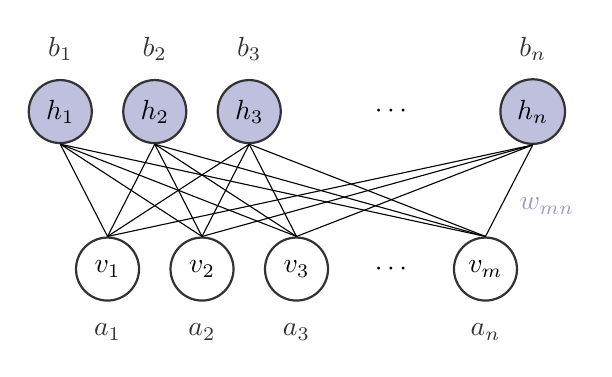
\begin{tikzpicture}
\tikzset{cir/.style={circle,draw=black!80,thick,minimum size=0.8cm},y=0.6cm,font=\sffamily}

\definecolor{bluebell}{rgb}{0.5, 0.5, 0.74}

\tikzset{cirblue/.style={circle,draw=black!80,thick,
    fill=bluebell!50,minimum size=0.8cm},y=0.6cm,font=\sffamily}

\begin{scope}[rotate=90]
\node[cir] (b1) at (0,0) {$v_1$};
\node[cir] (b2) at (0,-1*2) {$v_2$};
\node[cir] (b3) at (0,-2*2) {$v_3$};
\node[cir] (b4) at (0,-4*2) {$v_m$};
\node[cirblue] (c1) at (2,1) {$h_1$};
\node[cirblue] (c2) at (2,-1*2+1) {$h_2$};
\node[cirblue] (c3) at (2,-2*2+1) {$h_3$};
\node[cirblue] (c4) at (2,-4*2-1) {$h_n$};

\draw (-0.8, 0) node[black!80] {$a_1$};
\draw (-0.8, -1*2) node[black!80] {$a_2$};
\draw (-0.8, -2*2) node[black!80] {$a_3$};
\draw (-0.8, -4*2) node[black!80] {$a_n$};
\draw (2.8, 1) node[black!80] {$b_1$};
\draw (2.8, -1*2+1) node[black!80] {$b_2$};
\draw (2.8, -2*2+1) node[black!80] {$b_3$};
\draw (2.8, -4*2-1) node[black!80] {$b_n$};
\draw (0.8, -4*2-1.3) node[bluebell!80] {$w_{mn}$};

\foreach \i in {0,2} {
    \draw (\i,-3*2) node {$\cdots$};
}

\foreach \cnto in {1,2,3,4} {
    \foreach \cntt in {1,2,3,4} {
        \draw [-] (b\cnto.north)--(c\cntt.south);
    }
}

\end{scope}
\end{tikzpicture}
    \caption{Schematics of an RBM. Modified from the code found in \cite{stwind2020gist}.}
    \label{fig:rbm}
\end{figure}